\apendice{Documentación técnica de programación}

\section{Introducción}

	La idea de este apartado es marcar los pasos a seguir para que cualquier persona que decidiese escalar este trabajo pudiera ejecutarlo sin problema en su equipo. Es importante aclarar que Flutter establece una serie de requirimientos específicos que son de vital importancia para que todo funcione correctamente.

\section{Estructura de directorios}

	La estructura de directorios puede verse representada en la Figura \ref{fig:directorios}. Aunque muchas de las carpetas se crean automáticamente a la hora de crear el proyecto, destacan distintos archivos y directorios creados para la realización del trabajo. Hay que añadir que si no se comentan de manera específica significa que no son archivos donde se hayan realizado cambios y, por consiguiente, no son necesarios tocar si se quisiera escalar la aplicación.
	
\begin{figure}[H]
    \centering
    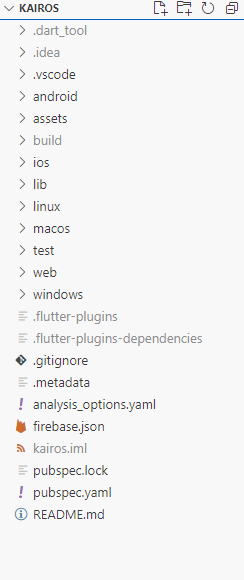
\includegraphics[width=0.5\linewidth]{img/directorios.png}
    \caption{Diseño de aplicar a una subasta y predicción de precio}
    \label{fig:directorios}
\end{figure}

	En la carpeta \emph{assets} se encuentran arhivos de diversos tipos que son necesarios para la realización de la aplicación. En mi caso, la carpeta contiene los siguientes archivos:
	\begin{enumerate}
		\item \textbf{databasewatches.csv :} archivo de extensión csv utilizado para el entrenamiento del modelo de predicción de precios y para cargar los desplegables de campos como \emph{brand}, \emph{model} y \emph{condition} entre otros. Más adelante veremos como se ha conseguido tal tarea.
		\item \textbf{kairoswallpaper.png :} imagen utilizada para establecer el fondo decorativo de la aplicación.
	\end{enumerate}
	
	En la carpeta \emph{lib} encontramos los scripts que han dado vida a la aplicación. Dentro de ella se han creado subdirectorios para seguir un orden y estructura claro. En este caso, los directorios han sido:
	\begin{enumerate}
		\item \textbf{models:} recoge los modelos de la aplicación.
		\item \textbf{views:} recoge los scripts con las vistas y controladores de la aplicación.
		\item \textbf{settings:} recoge scripts con funciones necesarias para traer datos de archivos presentes en la carpeta \emph{assets}.
	\end{enumerate}
	
	Por último, uno de los archivos más importantes es \emph{pubspec.yaml}, donde se definen todas las dependencias con sus versiones necesarias para compilar el programa.

\section{Manual del programador}

	Una vez explicado todo lo que uno debe saber antes de adrentarse en el proyecto, se procede a explicar cómo se ha programado la aplicación.
	
	En la carpeta \emph{models} se encuentran los tres scripts con extensión ``.dart'' que hacen el papel de modelos. Ya se pudo ver en la Figura \ref{fig:db5} y la Figura \ref{fig:db6} que era necesario entablar la comunicación con la base de datos y cómo debía hacerse.
	
	Con esto visto, solo queda explicar las clases ``AuctionRepository'', ``UserRepository'' y ``WatchRepository''. Todas estas clases manejan las operaciones de creación, lectura, actualización y eliminación de objetos según se necesitó para afrontar los requisitos establecidos. Sin embargo, una cosa fundamental que comparten las tres es la instancia de Firebase Firestore dentro de la clase para poder llevar todas estas a cabo, tal y como se representa en la Figura \ref{fig:instanciaFirebase}.

\imagen{instanciaFirebase}{Definición de atributo Firestore}

	Ya que todas las funciones están comentadas y explicar todo haría de este informe una novela, me quiero quedar con cómo se han realizado funciones de consulta de datos a la base de datos. En el caso del modelo ``user.dart'', se necesitó una función que devolviese el dinero de un usuario pasando como parámetro el correo electrónico de este, tal y como se representa en la Figura \ref{fig:consultaMonedero}.
	
\imagen{consultaMonedero}{Forma de consulta de datos a base de datos}

	La forma de consultar datos a base de datos nos obliga, en este caso, a definir una función asíncrona que devolverá eventualmente un entero. En cuanto a la parte de la consulta, se debe especificar la colección a la que se quiere acceder (recordemos que lo que siempre hemos conocido como tablas, aquí son colecciones), la condición que debe cumplir, y limitamos a uno el resultado porque solo debemos recibir un único valor (en este caso la cantidad del dinero asociado a ese correo electrónico). El ``.get()'' será el encargado de devolvernos un ``QuerySnapshot'' con los resultados de la consulta. 
	
	La siguiente comprobación simplemente nos asegura que, si ``QuerySnapshot'' no llegó vacío, devuelva el valor \emph{wallet} del primer documento. Si algo hubiera salido mal, se lanzaría una excepción especificando que el usuario no fue encontrado.
	
	Con las cosas claras de la parte de los modelos, pasamos a la parte de \emph{settings}. Como se ha explicado antes, esta carpeta se destinó a albergar funciones que pudieran ser comunes a varios \emph{scripts} y/o comunicaciones con otros archivos. En este caso, se destinó a albergar el \emph{script} donde se encuentra la función que permite cargar y procesar los datos del archivo con extensión ``.csv'' alojado en la carpeta \emph{assets}.
	
	Tal y como se representa en la Figura \ref{fig:cargaCSV}, la función va a cargar el archivo utilizando una función propia de Flutter y va devolver una lista de mapas con los datos procesados. Es importante tener en cuenta que la primera fila del archivo son los encabezados, por lo que se indica con ``csvTable.skip(1)''. 
	
\imagen{cargaCSV}{Función para extraer datos de dataset}

	En cuanto a las vistas, las funciones quedan explicadas en el código con distintos comentarios donde sean necesarios. Sin embargo, existen ciertas funciones que conviene dejar explciadas en este informe por si surgiese cualquier duda.
	
	Como podemos apreciar en la Figura \ref{fig:responsive}, todos los textos, botones e imágenes de la aplicación van a compartir semejanzas con ella. Es cierto que podría haberse utilizado funciones \emph{responsive} propias de la herramienta, pero durante la realización vimos que afeaba la interfaz ya que los botones tendían a ocupar el largo de la pantalla y, en monitor, no quedaba bonito. Por esta razón, se ideó ajustar el tamaño de los distintos objetos antendiendo al largo de la pantalla.
	
\imagen{responsive}{Forma de hacer la aplicación responsive}

	Otro aspecto importante es la actualización de \emph{widgets} cada vez que viajabamos de una vista a otra y/o realizabamos acciones que necesitaran de un \emph{reload} de la ventana para visualizar los nuevos datos. Un caso lo tenemos en la vista ``home.dart'', donde queremos que el \emph{widget} que presenta el dinero del usuario, se actualice cada vez que viajamos a la venta home. Esto es lo que se representa en la Figura \ref{fig:estadoWallet}. 

\imagen{estadoWallet}{Forma de actualizar un widget}

	Muchas de las cosas predefinidas por Flutter no son intuitivas para el usuario, por lo que se pensó definir una función que controlase la forma de visualizar los mensajes informativos que se den a lo largo de la apliación. Para ello se utiliza la función presentada en la Figura \ref{fig:formaDialogos}, la cual consta de dos partes donde definimos el título del error y una descripción detallada de ello.
	
\imagen{formaDialogos}{Funcion para visualización de diálogos}

	Como hemos indicado en otros apartados, la aplicación cuenta con una llamada a una API, consulta que es necesario definir en el \emph{script} ``addwatch.dart''. Para ello, es importante previamente importar el paquete ``http'', el cual va a permitir que podamos lanzar la consulta, indicando la dirección de la API en la web (alojada en Render). Si el estado de la consulta es 200, todo habrá ido bien. En cambio, si no lo fuese, debemos tratar las excepciones tal y como se plantea en el código. Código en la Figura \ref{fig:llamadaAPI}.

\imagen{llamadaAPI}{Forma de hacer consulta a la API}

	En cuanto a las contraseñas, me pareció una buena idea incluir una función muy presente en muchas webs y aplciaciones: ocultar y mostrar la \emph{password}. Para ello, simplemente definí dos variables booleanas que marcaran si la contraseña se debía mostrar o no en función del pulso sobre el botón definido. Tal código se ve representado en la Figura \ref{fig:ocultarPassword} y la Figura \ref{fig:ocultarPassword2} respectivamente.

\imagen{ocultarPassword}{Variables booleanas para contraseña}
\imagen{ocultarPassword2}{Lógica de ocultar y mostrar contraseña}

	Otro concepto que puede no ser entendido es lo definido como ``regex''. Simplemente se conocen como expresiones regulares y su objetivo es marcar patrones para la manipulación de texto. Mediante su uso, se ha conseguido marcar las validaciones de campos como contraseña, número de cuenta o nombre del usuario, entre otros. Su programación de puede ver en la Figura \ref{fig:validaciones}.
	 
\imagen{validaciones}{Expresiones regulares}

	Por último, no me quería dejar una función importante a la hora de establecer los primeros pasos con Firestore Database. En el \emph{script} ``main.dart'', en la mayoría de casos, solo se recogen las rutas definidas en la aplicación. Sin embargo, al trabajar con esta base de datos, es necesario definir la función representada en la Figura \ref{fig:inicializacionBaseDeDatos} para que todo funcione correctamente.
	
\imagen{inicializacionBaseDeDatos}{Función que inicializa Firebase}


\section{Compilación, instalación y ejecución del proyecto}

	Para poder ejecutar el proyecto en nuestro equipo, es importante cumplir una serie de requisitos previos e instalar algún que otro programa. Para hacerlo de la manera más estructurada posible, se detallan a continuación los que seguí según munoncode \cite{instalacion:flutter}:
	
	\begin{enumerate}
		\item Entramos en sitio web oficial de Flutter \cite{flutter}.
		\item Pulsamos sobre el botón ``Get started''.
		\item Pulsamos sobre el icono de nuestro sistema operativo (en mi caso Windows)
		\item Pulsamos sobre el botón ``Mobile''. Nos llevará a una página con todos los pasos a seguir.
		\item Dentro de la página, buscamos la referencia a Visual Studio Code. Pulsamos sobre ella. Nos llevará la página oficial de Visual Studio Code.
		\item Pulsamos en ``Download'', pulsamos sobre nuestro sistema operativo e instalamos el programa.
		\item Dentro de Visual Studio Code, vamos al apartado ``Extensiones'' y descargamos ``Flutter''.
		\item Volvemos al sitio oficial de Flutter y descargamos Flutter.
		\item (Opcional) Crear en el disco local C una carpeta con el nombre \emph{dev} y guardar lo anterior en dicha carpeta nueva.
		\item Accedemos a la configuración de variables de entorno y añadimos en \emph{path} la ruta a la carpeta \emph{bin} del archivo Flutter descargado.
		\item (Paso de confirmación) Si en la consola escribimos el comando ``flutter'' y lo reconoce, la instalación se realizó correctamente.
		\item Volvemos a la página oficial de Flutter y buscamos la referencia a Android Studio. Pulsamos sobre ella, vamos a su sitio web y descargamos el programa.
		\item Una vez instalado, dentro de Android Studio seguimos la ruta \emph{Tools-Device Manager}. Aquí podrás crear el emulador que necesites.
		\item En consola, aceptar las licencias necesarias con el comando ``flutter doctor --android-license''
		\item En consola, escribimos ``flutter doctor''. Si todo va bien, todos los requisitos necesarios estarán aprobados.
	\end{enumerate}
	
	Con todos estos pasos previos, ya podemos descargar el proyecto. Para ello, se deben seguir los siguientes pasos:
	\begin{enumerate}
		\item Entramos en el repositorio de GitHub.
		\item Descargamos todo el repositorio y descomprimimos el archivo con extensión .zip
		\item Abrimos Visual Studio Code y abrimos la carpeta ``kairos''.
		\item Abrimos una terminal con la ruta de la carpeta y lanzamos comando ``flutter run''
		\item Nos da como opciones los navegadores disponibles. En mi caso, elijo Google Chrome.
	\end{enumerate}
	
	De esta forma, ya tendríamos el proyecto corriendo en nuestro navegador. Si queremos realizar cambios mientras sigue corriendo el programa, introducir en consola una ``r'' para actualizar.

\section{Pruebas del sistema}

	Como tal, no se han realizado pruebas unitarias y/o de sistema de manera automática. Sin embargo, si se ha tenido en cuenta durante la programación de la aplicación las distintas validaciones de los campos que tuvieran que ver con la entrada de datos del usuario.
	
	Para llegar a esto, es muy importante tener bien definidos los diagramas de secuencia y contemplar todos los casos posibles que podrían darse al utilizar la aplicación. De esta forma, podemos crear mensajes informativos para el usuario donde se explique de manera detallada cual es el problema de su acción y que solución debe adoptar. 
	
	Las pruebas realizadas de manera manual para la confirmación de que las acciones realizadas sean correctas son:
	\begin{enumerate}
		\item Durante el inicio de sesión, introducir datos erróneos y obtener mensaje de error.
		\item Durante el registro, introducir valores numéricos en los campos \emph{Name}, \emph{Surnames} y \emph{Country}. Se obtiene mensaje de error.
		\item Durante el registro, introducir campo \emph{Password} sin seguir directrices marcadas en requisitos. Se obtiene mensaje de error.
		\item Durante el registro, introducir la confirmación de contraseña distinta al campo \emph{Password}. Se obtiene mensaje de error.
		\item Aplicar a subastas sin dinero suficiente, bien por no poder afrontar todas las posibles ganadoras o por falta de dinero en su monedero.
		\item Tratar de eliminar una subasta donde existe una puja. Botón bloqueado.
		\item Tratar de eliminar y/o editar un reloj que se encuentra en subasta. Botones bloqueados.
		\item Comprobación de cambios de estado tanto en subasta como en relojes.
	\end{enumerate}